% =============================================================================
% Financial Innovation (Springer / SWUFE) - Research article
%
% Multiplicative Information Gating.
%
% Build:  pdflatex fininnov_mig  ->  bibtex fininnov_mig  ->  pdflatex x2
%
% Class notes (see SUBMISSION-NOTES.md): sn-jnl.cls needs manyfoot, xcolor and
% amsthm loaded explicitly or it fails at \begin{document}.  The sn-basic option
% reproduces Financial Innovation's author-date house style exactly.
% =============================================================================
\documentclass[pdflatex,sn-basic]{sn-jnl}

\usepackage{manyfoot}%
\usepackage{xcolor}%
\usepackage{graphicx}%
\usepackage{multirow}%
\usepackage{amsmath,amssymb,amsfonts}%
\usepackage{amsthm}%
\usepackage{mathrsfs}%
\usepackage[title]{appendix}%
\usepackage{textcomp}%
\usepackage{booktabs}%

% The Springer sample calls for thmstyleone/thmstyletwo, which this copy of the
% class does not define; they are declared here to match the published look
% (bold run-in head, italic body for results; upright body for remarks).
\newtheoremstyle{thmstyleone}{9pt}{9pt}{\itshape}{}{\bfseries}{.}{.5em}{}
\newtheoremstyle{thmstyletwo}{9pt}{9pt}{\normalfont}{}{\bfseries}{.}{.5em}{}

\theoremstyle{thmstyleone}%
\newtheorem{proposition}{Proposition}%
\theoremstyle{thmstyletwo}%
\newtheorem{remark}{Remark}%

\raggedbottom

% Every number quoted in the prose is a macro emitted by analysis/06_tables.py
% from the result files, so the text cannot drift away from the data.
% Auto-generated by analysis/06_tables.py -- do not edit by hand.
\newcommand{\NCompanies}{35}
\newcommand{\ScoredHeadlines}{134,037}
\newcommand{\PanelRows}{117,312}
\newcommand{\NewsRows}{48,261}
\newcommand{\PanelSessions}{3,521}
\newcommand{\PanelStart}{2010-01-05}
\newcommand{\PanelEnd}{2023-12-29}
\newcommand{\PrecAHOne}{51.5}
\newcommand{\AurcAHOne}{0.479}
\newcommand{\PrecPriceHOne}{51.2}
\newcommand{\AurcPriceHOne}{0.485}
\newcommand{\BaseRateHOne}{51.8}
\newcommand{\PrecRelfHOne}{51.4}
\newcommand{\AurcRelfHOne}{0.482}
\newcommand{\GapPriceHOne}{+0.37}
\newcommand{\GapPriceCIHOne}{[-1.26, +1.96]}
\newcommand{\GapPricePHOne}{0.685}
\newcommand{\GapRelfHOne}{+0.07}
\newcommand{\GapRelfCIHOne}{[-1.70, +1.83]}
\newcommand{\GapRelfPHOne}{0.938}
\newcommand{\PrecAHFive}{52.4}
\newcommand{\AurcAHFive}{0.472}
\newcommand{\PrecPriceHFive}{54.0}
\newcommand{\AurcPriceHFive}{0.473}
\newcommand{\BaseRateHFive}{53.3}
\newcommand{\PrecRelfHFive}{53.8}
\newcommand{\AurcRelfHFive}{0.472}
\newcommand{\GapPriceHFive}{-1.23}
\newcommand{\GapPriceCIHFive}{[-3.52, +1.13]}
\newcommand{\GapPricePHFive}{0.322}
\newcommand{\GapRelfHFive}{-0.83}
\newcommand{\GapRelfCIHFive}{[-3.10, +1.40]}
\newcommand{\GapRelfPHFive}{0.482}
\newcommand{\PrecAHTwentyOne}{59.7}
\newcommand{\AurcAHTwentyOne}{0.458}
\newcommand{\PrecPriceHTwentyOne}{59.0}
\newcommand{\AurcPriceHTwentyOne}{0.457}
\newcommand{\BaseRateHTwentyOne}{54.9}
\newcommand{\PrecRelfHTwentyOne}{59.1}
\newcommand{\AurcRelfHTwentyOne}{0.460}
\newcommand{\GapPriceHTwentyOne}{+0.01}
\newcommand{\GapPriceCIHTwentyOne}{[-0.74, +0.72]}
\newcommand{\GapPricePHTwentyOne}{1.000}
\newcommand{\GapRelfHTwentyOne}{+0.37}
\newcommand{\GapRelfCIHTwentyOne}{[-0.23, +0.97]}
\newcommand{\GapRelfPHTwentyOne}{0.252}
\newcommand{\BestAlphaHOne}{0.75}
\newcommand{\BestBetaHOne}{0.00}
\newcommand{\BestICHOne}{0.0225}
\newcommand{\UnitICHOne}{0.0210}
\newcommand{\PureICHOne}{0.0209}
\newcommand{\BestAlphaHFive}{0.00}
\newcommand{\BestBetaHFive}{0.00}
\newcommand{\BestICHFive}{0.0156}
\newcommand{\UnitICHFive}{0.0126}
\newcommand{\PureICHFive}{0.0156}
\newcommand{\BestAlphaHTwentyOne}{0.75}
\newcommand{\BestBetaHTwentyOne}{1.25}
\newcommand{\BestICHTwentyOne}{0.0094}
\newcommand{\UnitICHTwentyOne}{0.0049}
\newcommand{\PureICHTwentyOne}{0.0081}
\newcommand{\StaleNuBeta}{-0.033}
\newcommand{\StaleNuT}{-6.51}
\newcommand{\StaleMuBeta}{-0.022}
\newcommand{\StaleMuT}{-3.91}
\newcommand{\AbsRetNuBps}{-26.3}
\newcommand{\AbsRetNuT}{-8.69}
\newcommand{\AbsRetMuBps}{54.3}
\newcommand{\AbsRetMuT}{12.70}
\newcommand{\PartialNuStale}{-0.014}
\newcommand{\PartialMuStale}{-0.014}
\newcommand{\DenseNuStale}{-0.155}
\newcommand{\DenseMuStale}{-0.157}
\newcommand{\StaleN}{133,933}
\newcommand{\AbsRetN}{130,828}
\newcommand{\NuPeakDecile}{4}
\newcommand{\NuAtPeak}{0.230}
\newcommand{\NuAtStalest}{0.167}
\newcommand{\NuAtFreshest}{0.093}
\newcommand{\ICCNu}{0.565}
\newcommand{\ICCMu}{0.727}
\newcommand{\ICCS}{0.779}
\newcommand{\RetestN}{250}


\begin{document}

\title[Validating multi-axis language-model features]{Asking a language model for
three scores does not give you three measurements: a validity check for
multi-axis text features, and what it costs to skip it}

\author*[1]{\fnm{Anandkumar} \sur{Pardeshi}}\email{anand.pardeshi@fcrit.ac.in}
\author[2]{\fnm{Sujata} \sur{Deshmukh}}\email{sujata.deshmukh@fragnel.edu.in}

\affil*[1]{\orgdiv{Department of Computer Science and Engineering},
  \orgname{Fr.\ C.\ Rodrigues Institute of Technology, University of Mumbai},
  \orgaddress{\city{Vashi, Navi Mumbai}, \country{India}}}

\affil[2]{\orgdiv{Department of Computer Engineering},
  \orgname{Fr.\ C.\ Rodrigues College of Engineering, University of Mumbai},
  \orgaddress{\city{Bandra, Mumbai}, \country{India}}}

% -----------------------------------------------------------------------------
\abstract{Practitioners increasingly prompt a language model for several
conceptually distinct scores per document and build features that assume those
scores measure different things. We show that this assumption can fail silently,
give a cheap diagnostic that detects the failure before any model is fitted, and
document what skipping it costs. The diagnostic is to name an external criterion
for each axis in advance and check that each axis tracks its own criterion rather
than its neighbour's; it requires no labelled data and, in our case, no additional
model calls. We demonstrate on a three-axis decomposition of financial news into
polarity, novelty and materiality, combined multiplicatively so that any near-zero
factor vetoes the signal --- a design we also characterise axiomatically, showing
that continuity, strict monotonicity and ratio-scale separability force the
combiner into the Cobb--Douglas family $s\,\nu^{\alpha}\mu^{\beta}$ whose
exponents the axioms leave free. Scoring \ScoredHeadlines\ headlines for
\NCompanies\ US-listed companies, the diagnostic fails: novelty and materiality
correlate at 0.871, and only materiality survives validation, predicting absolute
market-adjusted returns at $t=\AbsRetMuT$, while novelty carries no information
about mechanical staleness beyond what materiality already carries. Two of the
three axes are one latent judgement reported twice. The downstream consequences
follow exactly: freely estimated exponents place the materiality elasticity at
zero, the gated aggregate predicts returns no better than plain, count-weighted or
relevance-filtered polarity, and adding it to a walk-forward selective forecaster
moves precision at fixed coverage by between $-1.2$ and $+0.4$ percentage points
with every interval containing zero. The surviving axis measures magnitude rather
than direction, which a signed product cannot use --- a diagnosis available in
advance from the validity check alone.}

\keywords{Construct validity, Large language models, Feature engineering,
Sentiment analysis, Financial text}

\maketitle

% =============================================================================
\section{Introduction}\label{sec:intro}
% =============================================================================

Instruction-tuned language models have made a particular move cheap: instead of
extracting one score from a document, ask for several. A single prompt can request
sentiment, urgency and credibility from a support ticket; severity, novelty and
confidence from a clinical note; or, as here, polarity, novelty and materiality
from a news headline. The scores come back well-formed, on the requested scales,
and looking exactly like the distinct quantities that were asked for. Downstream
they are treated as distinct: combined, weighted, interacted, used as separate
features.

This paper is about a failure mode of that move. \emph{Asking for $k$ conceptually
distinct scores does not guarantee $k$ distinct measurements.} A model may return
one latent judgement dressed in $k$ labels, and nothing in the output reveals it:
the scores vary, they correlate imperfectly, they respond sensibly to examples, and
they are perfectly reproducible. The failure is silent, it is invisible in any
internal consistency check, and it propagates into every feature built on top of
it. Because the axes are correlated but not identical, even a careful analyst
looking at a correlation matrix may conclude they are distinct-but-related rather
than one thing measured twice.

The remedy we argue for is old and borrowed: \emph{convergent validity}. Before
building features, name for each axis an external criterion it must track if it
measures what its label claims, then check that each axis tracks its own criterion
rather than merely its neighbour's. The check needs no labelled data, and in our
case it needed no additional model calls, since both criteria were computable from
data already in hand. It is cheap enough to run first, and running it first would
have saved the entire modelling exercise that follows.

We demonstrate on a concrete design from financial text analysis, chosen because
it is one we built, believed in, and can therefore report against without
charity. A large class of decision systems reads news and acts on it, scoring each
item for sentiment polarity and averaging \citep{tetlock2007, tetlock2008,
antweiler2004, loughran2011, loughran2016}. Polarity answers only one question ---
is this good or bad? --- and is silent on two others any desk asks reflexively: is
the item \emph{new}, or a restatement of something priced weeks ago; and does it
\emph{bear on value}, or is it cosmetic? Both omissions are documented to matter:
investors underreact to stale news that recycles old information
\citep{tetlock2011}, and separating relevant from irrelevant news sharply changes
the measured information content of a news flow \citep{boudoukh2019}.

This paper takes a textual event to have three separable properties, each acting
on price through a different channel: \emph{polarity}, the sign and size of the
implied value change; \emph{novelty}, how much genuinely new information the item
carries relative to the market's prior; and \emph{materiality}, how sensitive
fundamental value is to the event, independent of sign or freshness.
\emph{Multiplicative information gating} combines them as a product, which
behaves like a soft logical AND: a stale or immaterial item produces a signal
near zero however extreme its polarity, so a single weak factor vetoes the event.

Who supplies the three scores? Dictionaries handle polarity passably
\citep{loughran2011} but novelty and materiality need world knowledge, which is
why they have historically come from commercial data vendors. An instruction-tuned
language model, prompted with fixed numerical anchors and memoised for
determinism, supplies all three at scale without a licence --- and it is exactly
this convenience that makes the validity question urgent, because the cost of
adding an axis has fallen to almost nothing while the cost of a spurious axis has
not.

The validity check fails on this design, and the rest of the paper is the audit
trail of what that failure costs. We race the product against plain polarity,
filtered polarity, count-weighted polarity and an additive combiner; we estimate
the exponents of the three axes freely rather than assuming them; and we fit a
walk-forward selective forecaster with and without the gated signal. Every one of
those results is consistent with, and predictable from, the diagnostic that could
have been run at the outset.

The framework is coupled to a decision stage, because a forecaster operating near
the efficient-market limit \citep{fama1970} is wrong about direction most of the
time and therefore owes its user two things: a probability that means what it
says, and the discipline to abstain when conviction is low
\citep{chow1970,geifman2017}. The same veto logic that suppresses an immaterial
headline at the text stage suppresses a low-conviction name at the decision
stage.

Our contributions are as follows.

\begin{enumerate}
\item \textbf{A validity protocol for multi-axis language-model features}
  (Section~\ref{sec:protocol}). For each axis, name an external criterion in
  advance, then test whether the axis tracks its own criterion \emph{conditional
  on the other axes}. The conditioning does the work: raw correlations with a
  criterion look reassuring even when one latent judgement drives every axis. The
  protocol needs no labelled data and, here, no additional model calls.
\item \textbf{Evidence that the failure is real, and a worked diagnosis}
  (Section~\ref{sec:validity}). On \ScoredHeadlines\ headlines for \NCompanies\
  US-listed companies, two of three axes collapse: novelty and materiality
  correlate at $0.871$, and only materiality survives validation --- it predicts
  absolute market-adjusted returns at $t=\AbsRetMuT$, while novelty carries no
  information about mechanical staleness beyond what materiality already carries.
\item \textbf{A measurement of what skipping the check costs}
  (Sections~\ref{sec:univariate}--\ref{sec:selective}). Freely estimated exponents
  put the materiality elasticity at zero; the gated aggregate predicts returns no
  better than plain, count-weighted or relevance-filtered polarity; and adding it
  to a walk-forward selective forecaster moves precision at fixed coverage by
  between $-1.2$ and $+0.4$ percentage points, every interval containing zero.
  Each result is predictable from the diagnostic alone.
\item \textbf{A characterisation of the design under test}
  (Section~\ref{sec:model}). We prove a veto bound (Proposition~\ref{prop:veto})
  and show (Proposition~\ref{prop:rep}) that continuity, strict monotonicity, sign
  fidelity and ratio-scale separability force the combiner into the Cobb--Douglas
  family $\mathrm{sign}(s)\,|s|^{\alpha_0}\nu^{\alpha}\mu^{\beta}$. The axioms do
  \emph{not} pin the exponents, which is what makes them estimable and the design
  falsifiable rather than definitional.
\item \textbf{Deployment evidence on calibration and abstention}
  (Section~\ref{sec:live}) from a live, append-only ledger of 621 resolved
  interval forecasts, including a diagnosed and repaired calibration failure. It
  concerns the decision stage and is kept strictly separate from the claims about
  text, which it cannot support.
\end{enumerate}

A note on how to read this paper. We proposed the decomposition, built the
instrument, believed in it, and then found against it. The framework is reported
in full alongside the evidence that it does not pay, because a design this
intuitive will be reinvented, and because the useful artefact is not the verdict
but the check that reaches it in an afternoon rather than a year.

% =============================================================================
\section{Related work}\label{sec:related}
% =============================================================================

\subsection{Text, tone and returns}

Tetlock \citep{tetlock2007} linked pessimistic media tone to downward price
pressure and subsequent reversal; \citet{tetlock2008} showed that negative
language in firm-specific news predicts earnings and returns.
\citet{antweiler2004} studied message boards, and \citet{loughran2011}
demonstrated that finance-specific word lists matter because general-purpose ones
systematically mislabel domain terms, a point developed in their later survey
\citep{loughran2016}. \citet{garcia2013} showed the effect of tone is
state-dependent, concentrated in recessions. Supervised and neural text models
improve on dictionaries \citep{ke2019,huang2023}, and machine learning is now
standard in empirical asset pricing \citep{gu2020}. What unites this literature
is that the per-item output is a scalar polarity; novelty and materiality, when
handled at all, are handled by ad hoc pre-filters.

\subsection{Relevance and novelty are established constructs, not new ones}

We want to be explicit about prior art, because the decomposition proposed here
is not the first attempt to look past polarity. Commercial news analytics have
scored relevance and event novelty for well over a decade: RavenPack's feeds
attach a relevance score, an event novelty score and an event sentiment score to
each item, and a large empirical literature filters on exactly those fields
before running its tests. On the academic side, the novelty axis has a canonical
antecedent in \citet{tetlock2011}, who separates genuinely new stories from
reprints of stale information and finds that investors react to the stale
component; \citet{boudoukh2019} show that identifying which news is
\emph{relevant} materially changes measured information content;
\citet{dang2015} study commonality in news flow across markets; and
\citet{kelly2021} treat which text gets written at all as an object of study.
\citet{hillert2014} document how media coverage intensity interacts with
momentum, and \citet{dellavigna2009} show that the same information moves prices
differently depending on when attention is available to receive it.

Against that background we make no claim to have discovered novelty or
materiality as constructs. Our residual contributions are narrower and, we think,
defensible: (i) the three axes are produced \emph{zero-shot by a general-purpose
language model under a published prompt}, which replaces a licensed proprietary
feed with something any research group can reproduce and audit; (ii) they are
combined by a \emph{continuous product with estimated elasticities} rather than
used as hard pre-filter thresholds, which is how practitioners overwhelmingly use
relevance scores; and (iii) the functional form is derived rather than asserted,
and then tested against the alternatives on the same data.

\subsection{Language models as measurement instruments}

Instruction-tuned models emit structured numeric judgements from rubric-style
prompts \citep{brown2020}, and finance has adopted them quickly for return
prediction \citep{lopezlira2025} and for reading corporate policy
\citep{jha2024}. Their self-reported confidence, however, is imperfectly
calibrated and is perceived by users as better than it is \citep{steyvers2025}.
This motivates a deliberate division of labour in our design: we never ask the
model to forecast. We ask it only to \emph{decompose} an item along three
defined axes, a narrower and more checkable task, and we leave forecasting and
uncertainty quantification to a separate stage that can be calibrated against
outcomes.

\subsection{Calibration and selective prediction}

Modern classifiers are frequently miscalibrated \citep{guo2017}. Standard
remedies are Platt scaling \citep{platt1999} and isotonic regression
\citep{zadrozny2002}, assessed by expected calibration error and the Brier score
\citep{brier1950}. Stacking \citep{wolpert1992} complicates this by creating more
than one score distribution, a failure mode we diagnose and repair in
Section~\ref{sec:calib}. Abstention is an old idea \citep{chow1970} with a modern
theory \citep{geifman2017,elyaniv2010} and a distribution-free relative in
conformal prediction \citep{angelopoulos2023}. Financial machine learning remains
dominated by accuracy and area-under-the-curve reporting, which is fragile under
backtest overfitting \citep{bailey2017} and multiple testing
\citep{harvey2016,romano2005}; comparatively little of it reports whether the
probabilities can be trusted.

% =============================================================================
\section{The multiplicative information model}\label{sec:model}
% =============================================================================

\subsection{Events, axes and the event signal}

Let $e$ denote a textual event -- in our data, a news headline -- about an entity,
a listed equity. The event carries three scores:
\begin{itemize}
\item polarity $s(e)\in[-1,1]$, the sign and size of the implied value change;
\item novelty $\nu(e)\in[0,1]$, the surprise relative to the market's prior;
\item materiality $\mu(e)\in[0,1]$, the sensitivity of fundamental value to the
  event, independent of sign and of freshness.
\end{itemize}
The \emph{event signal} is their product,
\begin{equation}\label{eq:signal}
a(e)\;=\;s(e)\,\nu(e)\,\mu(e)\;\in[-1,1].
\end{equation}
Define \emph{relevance} $r(e)=\nu(e)\mu(e)$, so that $a(e)=s(e)\,r(e)$. The
economic reading is a first-order decomposition: the expected price move is the
product of a direction, a sensitivity and a surprise magnitude. Additive
sentiment retains only the first, which is why it overreacts to loud but stale or
immaterial items.

\subsection{Aggregation}

To aggregate the events $\mathcal{E}$ touching one entity in one period we use a
relevance-weighted mean, restricted to events clearing a materiality floor
$\mu_0$:
\begin{equation}\label{eq:agg}
A\;=\;\frac{\sum_{e\in\mathcal{E}:\,\mu(e)\ge\mu_0} r(e)\,a(e)}
           {\sum_{e\in\mathcal{E}:\,\mu(e)\ge\mu_0} r(e)}
 \;=\;\frac{\sum r(e)^2\,s(e)}{\sum r(e)}.
\end{equation}
Relevance therefore enters twice, once inside the event signal and once as the
weight, so a novel and material item dominates quadratically while cosmetic
chatter is suppressed. We set $\mu_0=0.15$, the value used by the deployed
system; Section~\ref{sec:robust} reports sensitivity to it.

\subsection{Two properties of the product form}

\begin{proposition}[Veto bound]\label{prop:veto}
For every event $e$,
$\;|a(e)|\le\min\{\,|s(e)|,\ \nu(e),\ \mu(e)\,\}$.
In particular $a(e)=0$ whenever any single factor is zero, and the aggregate of
Eq.~\eqref{eq:agg} satisfies $|A|\le\max_{e}|s(e)|$.
\end{proposition}

\begin{proof}
Each factor has modulus at most one and $\nu,\mu\ge0$, so
$|a(e)|=|s(e)|\,\nu(e)\,\mu(e)$ is a product of three numbers of modulus at most
one; such a product cannot exceed the modulus of any one of them, which gives the
per-event bound and the zero case. For the aggregate,
\[
|A|\;\le\;\frac{\sum_e r(e)^2\,|s(e)|}{\sum_e r(e)}
   \;\le\;\max_e|s(e)|\cdot\frac{\sum_e r(e)^2}{\sum_e r(e)}
   \;\le\;\max_e|s(e)|,
\]
where the last step uses $\sum_e r(e)^2\le(\max_e r(e))\sum_e r(e)\le\sum_e r(e)$
because every $r(e)\in[0,1]$. The weights are non-negative but sub-stochastic, so
the aggregate contracts the polarities toward zero and never amplifies them.
\end{proof}

Proposition~\ref{prop:veto} is what ``a single weak factor vetoes the event''
means formally: a stale ($\nu\!\to\!0$) or immaterial ($\mu\!\to\!0$) item is
capped near zero however extreme its polarity. No additive combination has this
property, since a weighted sum $\alpha s+\beta\nu+\gamma\mu$ is generally nonzero
when one term vanishes.

The second question is why a product rather than any other veto-respecting form.
An earlier version of this argument assumed that scaling any one axis by
$\lambda$ scales the combiner by $\lambda$, which is close to assuming the
conclusion. The following statement replaces that assumption with the standard
conditions of conjoint measurement \citep{debreu1960,gorman1968,krantz1971} plus
the observation that each axis is measured on a ratio scale.

\begin{proposition}[Representation]\label{prop:rep}
Let $f:[-1,1]\times(0,1]\times(0,1]\to[-1,1]$ satisfy
\begin{description}
\item[(A0)] \emph{normalisation}: $f(1,1,1)=1$;
\item[(A1)] \emph{sign fidelity}: $\operatorname{sign}f(s,\nu,\mu)=\operatorname{sign}(s)$;
\item[(A2)] \emph{veto}: $f=0$ whenever any of $|s|,\nu,\mu$ equals $0$;
\item[(A3)] \emph{regularity}: $f$ is continuous and, on the interior,
  $|f|$ is strictly increasing in each of $|s|,\nu,\mu$;
\item[(A4$'$)] \emph{ratio-scale separability}: for each argument there is a
  function $h$ of one variable such that multiplying that argument by
  $\lambda\in(0,1]$ multiplies $|f|$ by $h(\lambda)$, whatever the values of the
  other two arguments.
\end{description}
Then there exist exponents $\alpha_0,\alpha,\beta>0$ with
\begin{equation}\label{eq:cd}
f(s,\nu,\mu)\;=\;\operatorname{sign}(s)\,|s|^{\alpha_0}\,\nu^{\alpha}\,\mu^{\beta}.
\end{equation}
\end{proposition}

\begin{proof}
Work on the positive orthant $|s|,\nu,\mu\in(0,1]$ and write $F=|f|$. Fix the
second and third arguments. By (A4$'$) there is $h_0$ with
$F(\lambda x,\nu,\mu)=h_0(\lambda)F(x,\nu,\mu)$ for all admissible
$\lambda,x$. Applying this twice,
\[
h_0(\lambda_1\lambda_2)F(x,\nu,\mu)=F(\lambda_1\lambda_2 x,\nu,\mu)
 =h_0(\lambda_1)F(\lambda_2x,\nu,\mu)=h_0(\lambda_1)h_0(\lambda_2)F(x,\nu,\mu),
\]
and since $F>0$ on the interior, $h_0$ satisfies the multiplicative Cauchy
equation $h_0(\lambda_1\lambda_2)=h_0(\lambda_1)h_0(\lambda_2)$. By (A3) $h_0$ is
continuous and positive, so its only solutions are the power functions
$h_0(\lambda)=\lambda^{\alpha_0}$ \citep{aczel1966}, with $\alpha_0>0$ because
$F$ is strictly increasing in its first argument. Setting $x=1$ gives
$F(\lambda,\nu,\mu)=\lambda^{\alpha_0}F(1,\nu,\mu)$. Repeating the argument for
the second and third arguments yields exponents $\alpha,\beta>0$ and
$F(|s|,\nu,\mu)=|s|^{\alpha_0}\nu^{\alpha}\mu^{\beta}F(1,1,1)$, and (A0) fixes
$F(1,1,1)=1$. Restoring the sign by (A1) gives Eq.~\eqref{eq:cd}. Continuity
extends the representation to the closed domain, where (A2) is then automatic
because all three exponents are strictly positive.
\end{proof}

\begin{remark}\label{rem:notpinned}
Proposition~\ref{prop:rep} delivers the \emph{family}, not a member of it. The
combiner of Eq.~\eqref{eq:signal} is the special case
$\alpha_0=\alpha=\beta=1$, and nothing in (A0)--(A4$'$) selects it. This is
deliberate. The axioms say that the three axes act on separate multiplicative
scales and cannot compensate for one another, which is the substantive claim; the
elasticities with which they act are an empirical matter, and
Section~\ref{sec:exponents} estimates $\alpha$ and $\beta$ freely and tests
$H_0\!:\alpha=\beta=1$ rather than assuming it. Proposition~\ref{prop:veto} holds
for every member of the family in the weaker form
$|f|\le\min\{|s|^{\alpha_0},\nu^{\alpha},\mu^{\beta}\}$, so the veto survives
whatever the exponents turn out to be.
\end{remark}

% =============================================================================
\section{Data and methods}\label{sec:methods}
% =============================================================================

\subsection{Two separate bodies of evidence}\label{sec:evidence}

The paper draws on two datasets that are kept strictly apart, because they answer
different questions and come from different markets.

\paragraph{A live deployment ledger (Indian large caps).} The forecasting system
described in Sections~\ref{sec:calib} and \ref{sec:gate} is deployed on liquid
National Stock Exchange of India (NSE) large-capitalisation equities. Since April
2026 it has written every issued forecast to an append-only ledger -- entity,
timestamp, target date, point forecast, interval, nominal confidence, directional
probability and horizon -- with each row later stamped with the realised price and
outcome. Rows are scored at first look and never retro-edited. This ledger
supplies the evidence on interval coverage and calibration in
Section~\ref{sec:live}. It cannot speak to the value of the text decomposition,
because it stores no per-event return labels and its history is far too short to
fit anything.

\paragraph{A large historical news panel (US equities).} To test the
decomposition itself we need a long panel with dense per-item news and clean
price data. We use FNSPID \citep{dong2024}, a public corpus of time-stamped
financial news headlines keyed to tickers. From the subset of symbols with
usable price histories we take the SYMBOL\_UNIVERSE best-covered names and remove
exchange-traded funds, for which ``the sensitivity of this firm's fundamental
value to the event'' has no clean meaning. That leaves N\_COMPANIES operating
companies, deliberately close in number to the 54-name universe of the NSE
deployment. Prices are split- and dividend-adjusted daily bars; returns are
market-adjusted using per-symbol betas against SPY fitted on the training window
only, and a Parkinson range estimator \citep{parkinson1980} supplies a volatility
proxy.

We state the obvious limitation at the outset rather than in a closing caveat:
\emph{the validation market is not the deployment market.} There is no historical
Indian headline corpus of comparable density available to us, so the question
``does multiplicative gating carry information?'' is answered on US data, and the
question ``does a calibrated selective forecaster behave as designed in
production?'' is answered on Indian data. Neither result is used to support a
claim about the other market.

\subsection{Scoring the three axes}\label{sec:scoring}

The axes are produced by an instruction-tuned large language model prompted as a
quantitative analyst and constrained to return a JSON array of
$\{\nu,\mu,s\}$ triples, one per headline, in input order. Three design choices
make the measurement reproducible.

First, the prompt fixes \emph{numerical anchors} on every axis. For novelty,
$0.0$ is an exact restatement of news priced weeks ago or a generic market list,
$0.2$ an in-line and widely expected result, $0.6$ an unexpected but modest
development and $1.0$ a sudden shock such as a surprise regulatory action. For
materiality, $0.0$ is boilerplate or a price-move round-up, $0.4$ a contract or
ruling worth a few percent of revenue, $0.8$ a transformative deal or guidance
reset and $1.0$ an existential event. For polarity the anchors run from $-1.0$
(fraud allegation) through $0.0$ (a neutral reshuffle) to $+1.0$ (a large
earnings beat or a takeover at a premium). Anchoring matters more here than in
ordinary sentiment work because the product in Eq.~\eqref{eq:signal} amplifies
disagreement on any single axis.

Second, every scored item is memoised in a content-addressed store keyed by the
SHA-1 hash of the entity and the normalised headline, so repeated runs are
deterministic and the full scoring history is auditable.

Third, the axes are scored \emph{zero-shot}: no labelled training data, no
fine-tuning and no market outcome enters the prompt, so the scores cannot encode
look-ahead information about the returns they are later used to predict.

The deployed Indian system uses Claude Haiku 4.5 for this role. The US validation
panel was scored with Gemini 3.1 Flash-Lite. Using different models in the two
settings is not ideal for comparability, but it does supply evidence on a
question that matters for the protocol's portability, namely whether the anchored
prompt is model-specific; Section~\ref{sec:reliability} reports test--retest
reliability of the axes.

\subsection{A validity protocol for multi-axis scores}\label{sec:protocol}

Before any feature is built from the three axes, we state the check that this
paper argues should come first. It is an application of convergent and
discriminant validity, standard in psychometrics and unusual in applied
text-as-data work, adapted to the situation where the ``instrument'' is a prompt.

\begin{enumerate}
\item \textbf{Name a criterion per axis, in advance.} For each axis, state an
  observable quantity that the axis must track \emph{if} it measures what its
  label claims, and that the other axes have no particular reason to track. The
  criterion must be computable without the axis itself. Here, novelty is assigned
  mechanical staleness --- lexical overlap with the same entity's recent coverage
  --- and materiality is assigned outcome magnitude, the absolute market-adjusted
  return.
\item \textbf{Test conditionally, not marginally.} Regress each criterion on all
  axes jointly, or equivalently examine partial correlations. This is the step
  that carries the diagnostic weight. If a single latent judgement drives every
  axis, each axis will show a respectable \emph{marginal} association with every
  criterion, and only the conditional test reveals that none of them adds anything
  to the others.
\item \textbf{Inspect the shape before summarising it.} A rank correlation is
  meaningless if the relationship is not monotone. We plot each axis against
  deciles of its criterion first, and only then report a coefficient.
\item \textbf{Control the mechanical confounds of the criterion.} A criterion
  computed from a comparison set inherits that set's properties; a document with
  few predecessors scores as novel by construction. The size of the comparison set
  enters as a control.
\item \textbf{Check that the criterion is the right \emph{kind} of quantity for
  the downstream task.} An axis can be valid and still useless: one that
  legitimately measures magnitude cannot sharpen a directional forecast. This step
  is what turns a validity result into a design decision.
\end{enumerate}

Two properties make this cheap enough to be worth doing routinely. Neither
criterion here required labelled data, and neither required additional model
calls: mechanical staleness is computed from the corpus already collected, and
outcome magnitude from prices already needed for the study. Note also that the
outcome criterion is used to validate the instrument and never as an input to any
signal --- checking whether a measurement means what it says against an outcome is
legitimate, whereas building the measurement from that outcome would not be.

\subsection{Aggregators raced against the product}\label{sec:baselines}

For every symbol-session with at least one headline we compute $A$ from
Eq.~\eqref{eq:agg} together with four competing aggregators and two ablations,
all built from the same scored events so that no comparison is confounded by
differences in the underlying text:

\begin{description}
\item[Mean polarity] $\overline{s}$, the standard additive recipe.
\item[Relevance-filtered polarity] the mean polarity of events clearing the
  materiality floor. This is the baseline that matters most, because it is what
  practitioners actually do with a vendor relevance score, and it captures much
  of the same information as the product.
\item[Count-weighted polarity] $\sum_e s(e)/\sqrt{|\mathcal{E}|}$, which rewards
  repeated coverage as a naive ``sum the sentiment'' pipeline implicitly does.
\item[Additive combiner] the mean of $(s+\nu+\mu)/3$: the natural
  non-multiplicative way to use exactly the same three inputs.
\item[Single-axis ablations] the same relevance-weighted aggregate built from
  $s\nu$ alone and from $s\mu$ alone, which isolate how much of the product's
  behaviour comes from each gate.
\end{description}

\subsection{Timing convention}\label{sec:timing}

Every headline carries a UTC publication stamp. It is converted to
America/New\_York and assigned to the session whose 16:00 ET close first follows
it, so the aggregate for session $d$ contains only information public before that
close and is used to predict returns realised from session $d+1$ onward. This
convention is applied uniformly and is the single most important guard in the
study: a related analysis in our own earlier work produced a spuriously
significant result that turned out to be a time-zone join artefact, and the
convention above was adopted after that diagnosis.

\subsection{From gated signal to calibrated probability}\label{sec:calib}

The aggregate $A$ is one feature among several entering a forecaster that also
sees price, momentum, trend, reversal and volatility features, and that emits per
name and horizon a point forecast, a price interval and a directional probability
$\hat p$. We treat the forecaster as a black box and study its calibration,
measured by the expected calibration error over $B$ equal-width bins,
\begin{equation}\label{eq:ece}
\mathrm{ECE}=\sum_{b=1}^{B}\frac{|G_b|}{N}\,
\bigl|\,\overline{y}_b-\overline{p}_b\,\bigr|,
\end{equation}
with $\overline p_b$ and $\overline y_b$ the mean predicted probability and mean
realised outcome in bin $b$, and by the Brier score
$N^{-1}\sum_i(\hat p_i-y_i)^2$ \citep{brier1950}.

The first deployed version of this model reported next-day up-probabilities
clustered near $0.80$ against a realised accuracy near $0.51$. The cause was a
stacking domain mismatch \citep{wolpert1992}: an isotonic calibrator had been
fitted on the out-of-fold \emph{average of the base learners} and was then
applied to the \emph{stacked} prediction, a different distribution, and the blend
itself was never calibrated. The repair is a three-stage procedure -- refit the
isotonic map on the base-average it was meant to correct, form the blend, then
fit a final Platt scaler \citep{platt1999} on a held-out fold and apply it to the
test and live rows. The general lesson is that a calibrator is bound to the
distribution it was fitted on, and stacking silently creates more than one.

\subsection{The conviction gate}\label{sec:gate}

Calibration makes $\hat p$ honest, not skilful. If short-horizon direction is
close to unpredictable, a calibrated probability sits near the base rate almost
everywhere and acting on every name is pointless. The remedy mirrors the
text-stage veto: act only when conviction clears a threshold. For a horizon of
$H$ sessions we emit an UP call when $\hat p\ge\tau^\star$ and abstain otherwise,
choosing $\tau^\star$ on training data as the smallest $\tau$ whose fired bucket
reaches a target precision while still firing at least a minimum fraction of the
time,
\begin{equation}\label{eq:tau}
\tau^\star=\min\bigl\{\tau:\ \operatorname{prec}(\tau)\ge \pi_0
\ \text{and}\ \phi(\tau)\ge\phi_0\bigr\},
\end{equation}
where $\operatorname{prec}(\tau)=\Pr[y=1\mid\hat p\ge\tau]$ and
$\phi(\tau)=\Pr[\hat p\ge\tau]$, with $\pi_0=0.60$ and $\phi_0=0.05$. The gate is
one-sided because confident DOWN calls are destroyed by the upward drift of
equities, so the system emits long-or-neutral signals only.

Reporting a single operating point invites the objection that $\tau^\star$ was
tuned to the number being reported. We therefore also report the full
\emph{risk--coverage curve} and its area (AURC): sorting predictions by
confidence and sweeping the threshold traces the selective risk accepted at each
coverage level, and the area under that curve summarises the whole trade-off
without reference to any threshold \citep{elyaniv2010,geifman2017}.

\subsection{Evaluation protocol and inference}\label{sec:inference}

All panel results are walk-forward by calendar year: for test year $Y$ the model
sees only sessions strictly before 1 January $Y$, the last 20\% of the training
sessions are held out to fit the probability calibrator and to choose
$\tau^\star$, and neither is ever selected on test data. Inference respects the
two dependence structures of a return panel: a market-wide shock hits every name
on the same date, and returns are persistent within a name. We therefore report
two-way clustered standard errors by date and symbol \citep{cameron2011},
cross-checked against Fama--MacBeth cross-sectional slopes with Newey--West
correction \citep{famamacbeth1973,neweywest1987}. Multi-session horizons are
evaluated on non-overlapping windows as the primary specification, and confidence
intervals for differences between models come from a block bootstrap that
resamples whole dates, preserving cross-sectional correlation.

% =============================================================================
\section{Results}\label{sec:results}
% =============================================================================

We report the results in the order a sceptical reader would want them: first
whether the instrument measures anything stable, then whether the three axes are
the separate things the model of Section~\ref{sec:model} assumes, then whether the
gated aggregate predicts returns, and only last whether it predicts them better
than the simpler recipes it is meant to replace. The answers are, in order: yes,
\emph{no}, yes, and no.

\begin{table}[htbp]
\caption{The two bodies of evidence. The validation panel answers whether the
decomposition carries information; the deployment ledger answers whether a
calibrated selective forecaster behaves as designed in production. They are drawn
from different markets and are never used to support claims about each other.}
\label{tab:data}
\begin{tabular}{@{}lll@{}}
\toprule
 & \textbf{Validation panel} & \textbf{Deployment ledger} \\
\midrule
Market & US listed equities & NSE India large caps \\
Source & FNSPID headline corpus & Live append-only forecast ledger \\
Entities & 35 operating companies & 7 names (live), 54 (walk-forward) \\
Span & 2010-01-05 to 2023-12-29 & 19 Apr 2026 to 12 Jun 2026 \\
Sessions & 3,521 & -- \\
Symbol-sessions & 117,312 & -- \\
\ldots with scored news & 48,261 & -- \\
Headlines scored & 134,037 & -- \\
Resolved forecasts & -- & 621 \\
Question answered & Does gating carry information? & Is the deployed system honest? \\
\botrule
\end{tabular}
\end{table}


\subsection{The measurement instrument}\label{sec:reliability}

Scoring \ScoredHeadlines\ headlines for \NCompanies\ companies over
\PanelStart\ to \PanelEnd\ yields axes with sensible central tendencies: mean
novelty $0.189$, mean materiality $0.157$ and mean polarity $0.039$, the last
confirming the mild positive skew that the news-tone literature reports. Two
properties of the instrument deserve comment before anything is built on it.

First, the model reports on a \emph{coarse grid} rather than a continuum: the mass
sits on multiples of $0.1$, visible as the discrete bars of
Figure~\ref{fig:axes}(a). This is a property of anchored prompting, not an
artefact of our aggregation, and it means the axes carry less resolution than
their $[0,1]$ range suggests.

Second, the scores are \emph{deterministic by construction}. Every item is
memoised under a hash of the entity and normalised headline, so the panel is
exactly reproducible from the cache. That is a property of the memoisation, not of
the model, so we also rescored a random subsample of \RetestN\ headlines with the
cache bypassed and a \emph{different} instruction-tuned model, which tests the
stronger and more useful claim that the anchored protocol is portable rather than
model-specific. Agreement is moderate and, tellingly, uneven across the axes:
the intraclass correlation is $\ICCS$ for polarity, $\ICCMu$ for materiality and
only $\ICCNu$ for novelty, with the event signal $a=s\nu\mu$ inheriting $0.601$.

The ordering matters for how the rest of the paper should be read. Polarity, the
axis with decades of instrument development behind it, is the one two independent
models agree on most; novelty, the axis on which the framework's distinctive claim
rests, is the one they agree on least. Any true multiplicative effect is therefore
being estimated through the noisiest available channel, and classical attenuation
would bias the measured contribution of gating toward zero. We return to this in
Section~\ref{sec:limits}, because it is the most credible non-trivial explanation
of the null results that follow. The subsample is small --- \RetestN\ headlines,
bounded by API quota rather than by design --- so these coefficients are
indicative rather than precise.

\subsection{The veto works, and the axes are not separable}\label{sec:descriptive}

The gate does exactly what Proposition~\ref{prop:veto} promises.
Table~\ref{tab:desc} shows that $56.3\%$ of events fall below the materiality
floor and are refused outright, and that $47.6\%$ of symbol-sessions carrying news
end up with an aggregate of exactly zero. The contraction is equally visible: the
standard deviation of the gated aggregate is $0.054$ against $0.154$ for mean
polarity, so gating removes about two-thirds of the cross-sectional dispersion of
the signal. Figure~\ref{fig:axes}(c) is the per-session version of the same
statement, with almost every point lying below the 45-degree line. On its own
terms, the mechanism is not in doubt.

The premise underneath it is. Multiplicative gating supposes that novelty and
materiality are \emph{separable} properties travelling through different channels.
In the measured data they are very nearly the same variable: the correlation
between $\nu$ and $\mu$ across all \ScoredHeadlines\ events is $\mathbf{0.871}$,
and Figure~\ref{fig:axes}(b) shows the joint mass collapsing onto the diagonal. An
item the model judges novel is almost always an item it judges material, and
conversely.

This single fact anticipates every result that follows. If two of the three axes
carry nearly the same information, then the second gate can add almost nothing
once the first has acted, the product cannot separate itself from simpler
combinations of the same inputs, and any attempt to estimate distinct elasticities
for $\nu$ and $\mu$ will be poorly identified. All three happen.

Two very different things could produce that correlation. It may be a fact about
the \emph{world} --- genuinely new firm news usually \emph{is} the consequential
news --- or a fact about the \emph{instrument}, an inability of the model to hold
two related concepts apart under one prompt. The two have opposite implications,
so the next subsection settles the question rather than leaving it open.

\subsection{Do the axes track anything outside themselves?}\label{sec:validity}

Each axis has an external criterion it must track if it measures what it claims,
and neither criterion requires further model calls.

\emph{Novelty should track mechanical staleness.} Following the stale-news
literature \citep{tetlock2011}, we measure how much a headline repeats what was
already written about the same ticker: one minus the maximum TF-IDF cosine
similarity to that ticker's headlines over the preceding thirty days. The
comparison set is strictly earlier in time, so the measure is causal and uses no
returns. It is available for $99.9\%$ of headlines, with a median of 38 prior
documents.

\emph{Materiality should track outcome magnitude.} Materiality is defined as the
sensitivity of value to an event \emph{regardless of direction}, so it should
predict the absolute market-adjusted return of the session. We stress that this
criterion is used only to validate the instrument and never as an input to any
signal: checking whether a measurement means what it says against an outcome is
legitimate, whereas building the measurement from that outcome would not be.

The results separate the two axes sharply, but not in the direction the framework
needs.

\textbf{Novelty fails its own criterion.} Figure~\ref{fig:validity}(a) plots both
axes against deciles of mechanical novelty, and the two curves are the same curve:
parallel, identically shaped, separated by a constant. The relationship is also
non-monotonic, rising from $\NuAtStalest$ at the stalest decile to $\NuAtPeak$ at
decile~\NuPeakDecile\ and then falling to $\NuAtFreshest$ at the most lexically
novel decile --- the model assigns its \emph{lowest} novelty to the headlines that
share least vocabulary with recent coverage. Controlling for materiality and for
the size of the comparison set, novelty's standardised coefficient on staleness is
$\StaleNuBeta$ ($t=\StaleNuT$) against materiality's $\StaleMuBeta$
($t=\StaleMuT$): statistically distinguishable from zero, but essentially the same
number, so novelty carries no staleness information that materiality does not
carry equally. The partial correlations tell the same story --- $\PartialNuStale$
for novelty given materiality, $\PartialMuStale$ for materiality given novelty ---
as does the dense subsample with at least twenty prior documents
($\DenseNuStale$ and $\DenseMuStale$, identical to three decimals).

\textbf{Materiality passes its own criterion, decisively.} Over \AbsRetN\ events,
a one standard deviation increase in materiality is followed by
$\AbsRetMuBps$ additional basis points of absolute market-adjusted return
($t=\AbsRetMuT$, clustered by date), while novelty enters the same regression with
the \emph{opposite} sign at $\AbsRetNuBps$ basis points ($t=\AbsRetNuT$). Whatever
common factor drives the $0.871$ correlation, the materiality label is the one
that aligns with a real external quantity; conditional on it, the novelty label
points the wrong way (Figure~\ref{fig:validity}(b)).

The verdict is therefore \emph{instrument}, and specifically the novelty axis. The
model is largely reporting a single latent ``importance'' judgement on both
channels; the channel labelled materiality happens to align with event magnitude,
and the channel labelled novelty does not measure novelty in the sense the
framework requires.

One implication deserves emphasis because it reaches past this instrument. The
valid axis, materiality, predicts the \emph{magnitude} of the move and not its
\emph{direction} --- which is exactly what its definition promises. But
Eq.~\eqref{eq:signal} multiplies it into a \emph{directional} signal. A quantity
that carries information about how large a move will be cannot improve a forecast
of which way it will go, and that, rather than any failure of measurement, is the
cleanest explanation for the materiality exponent estimating at zero in
Section~\ref{sec:exponents}. The decomposition would have a much better chance
against a volatility or absolute-return target than against a signed one.

\begin{figure}[htbp]
\centering
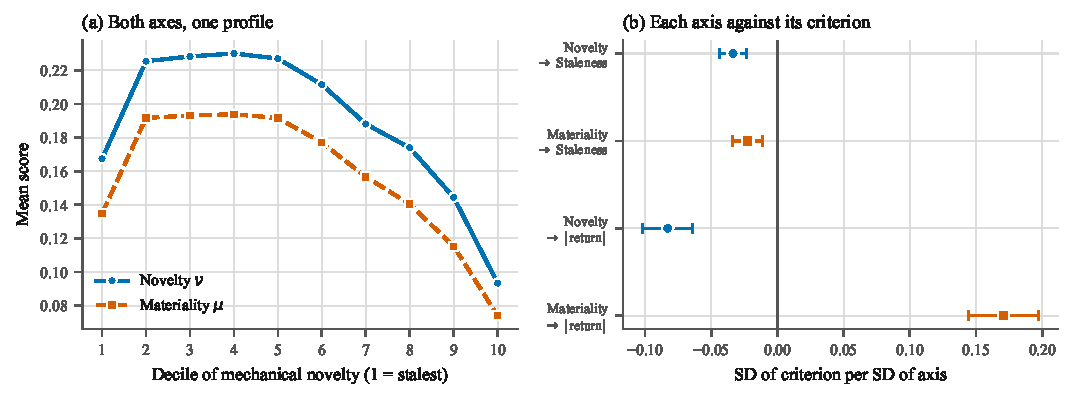
\includegraphics[width=\textwidth]{figures/fig6_convergent_validity.pdf}
\caption{Convergent validity of the two gates. (a) Mean novelty and mean
materiality across deciles of mechanical novelty: the two curves are parallel and
identically shaped, which is what one variable measured twice looks like, and both
are non-monotonic in mechanical novelty. (b) Standardised coefficients of each
axis on each criterion, in standard deviations of criterion per standard deviation
of axis, with 95\% intervals from date-clustered standard errors. Materiality
predicts absolute return strongly; novelty does not track mechanical staleness
beyond what materiality already tracks.}
\label{fig:validity}
\end{figure}

\begin{table}[htbp]
\caption{Descriptive statistics. Upper panel: the three axes and their products
at the level of the individual headline. Lower panel: the session-level
aggregators, computed on symbol-sessions carrying at least one scored headline.
The final column is the share of exactly-zero values, which is the share of
events or sessions the gate vetoes outright.}
\label{tab:desc}
\begin{tabular}{@{}lcccccc@{}}
\toprule
 & Mean & SD & p25 & Median & p75 & Zeros (\%) \\
\midrule
\multicolumn{7}{@{}l}{\textit{Panel A: per headline}} \\
Polarity $s$ & 0.039 & 0.207 & 0.000 & 0.000 & 0.200 & 52.0 \\
Novelty $\nu$ & 0.189 & 0.195 & 0.000 & 0.200 & 0.200 & 30.7 \\
Materiality $\mu$ & 0.157 & 0.166 & 0.000 & 0.100 & 0.200 & 34.4 \\
Relevance $r=\nu\mu$ & 0.058 & 0.100 & 0.000 & 0.020 & 0.060 & 35.0 \\
Event signal $a=s\nu\mu$ & 0.005 & 0.056 & 0.000 & 0.000 & 0.004 & 53.7 \\
\addlinespace
\multicolumn{7}{@{}l}{\textit{Panel B: per symbol-session}} \\
Gated signal $A$ & 0.006 & 0.054 & 0.000 & 0.000 & 0.008 & 47.6 \\
Relevance-filtered polarity & 0.042 & 0.195 & 0.000 & 0.000 & 0.200 & 48.4 \\
Mean polarity & 0.038 & 0.154 & 0.000 & 0.000 & 0.100 & 36.8 \\
Count-weighted polarity & 0.058 & 0.227 & 0.000 & 0.000 & 0.200 & 36.8 \\
Additive combiner & 0.118 & 0.107 & 0.033 & 0.100 & 0.167 & 17.7 \\
Novelty gate only ($s\nu$) & 0.017 & 0.091 & 0.000 & 0.000 & 0.040 & 36.7 \\
Materiality gate only ($s\mu$) & 0.013 & 0.079 & 0.000 & 0.000 & 0.040 & 37.2 \\
\botrule
\end{tabular}
\footnotetext{The correlation between novelty and materiality across all
events is 0.871: the two gates are close to the same variable, which is the
single fact behind most of what follows.}
\end{table}


\begin{figure}[htbp]
\centering
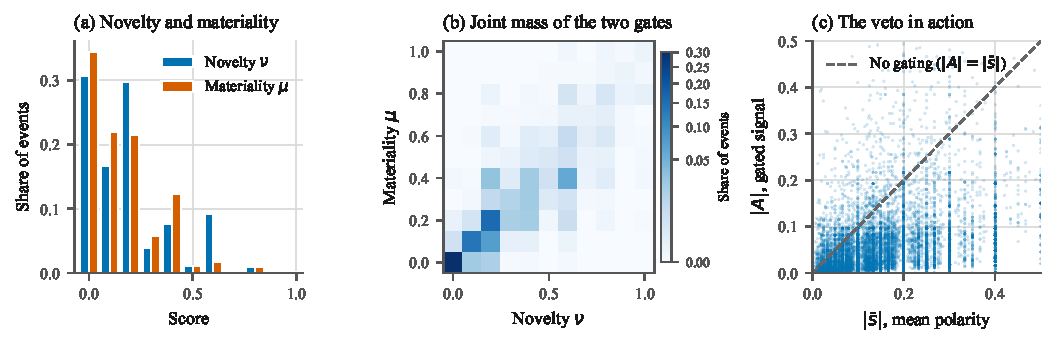
\includegraphics[width=\textwidth]{figures/fig1_axes_veto.pdf}
\caption{The three axes and the veto they implement, measured on
\ScoredHeadlines\ scored headlines. (a) Marginal distributions of novelty and
materiality; the model reports on a coarse grid, so the honest display is a
discrete bar chart. (b) Joint mass of the two gates, on a power-law colour scale
so the sparse high-novelty, high-materiality cells remain visible. (c) The gated
session aggregate $|A|$ against the mean absolute polarity $|\bar{s}|$ of the same
session: almost every point lies below the 45-degree line, which is
Proposition~\ref{prop:veto} in the data.}
\label{fig:axes}
\end{figure}

\subsection{Predictive content of the aggregators}\label{sec:univariate}

The gated aggregate does predict returns. At the one-session horizon a one
standard deviation move in $A$ is followed by $12.2$ basis points of
market-adjusted return, with a two-way clustered $t$ of $4.14$ and a
Fama--MacBeth $t$ of $3.70$; its rank information coefficient is $0.023$, averaged
over $2{,}548$ trading days with a Newey--West $t$ of $4.44$. At five sessions the
effect is $17.8$ basis points ($t=2.12$) on non-overlapping windows. By
twenty-one sessions nothing survives: every aggregator has $|t|<0.9$, which is
what one expects of headline-level information at a monthly horizon.

So the text carries signal. The question this paper exists to answer, though, is
whether the \emph{product} carries more of it than the recipes it is meant to
displace, and Table~\ref{tab:univariate} says it does not. At one session, mean
polarity earns a \emph{higher} $t$-statistic than the gated aggregate ($5.52$
versus $4.14$) on a nearly identical information coefficient ($0.021$ versus
$0.023$); count-weighted polarity produces a larger coefficient still
($14.1$ basis points) and the best information coefficient of the seven
($0.023$, $t=4.72$). Relevance-filtered polarity --- the hard-threshold recipe a
practitioner would actually deploy --- matches the product almost exactly
($10.0$ basis points, IC $0.023$). The one aggregator that clearly underperforms
is the additive combiner $(s+\nu+\mu)/3$ at $3.3$ basis points and IC $0.010$,
which is worth stating plainly: \emph{adding} the three axes is a bad idea, and to
that extent the argument against additive combination in
Section~\ref{sec:model} survives. It is the step from a filter to a product that
does not pay.

Figure~\ref{fig:univariate} makes the overlap visible. At the horizons where
anything is estimable, the confidence intervals of all seven aggregators sit on
top of one another.

\begin{table}[htbp]
\caption{Predictive regressions of forward market-adjusted returns on each
aggregator, one aggregator at a time. Regressors are standardised, so a
coefficient reads as basis points of forward return per one standard deviation of
signal. Standard errors are two-way clustered by date and symbol; horizons beyond
one session use non-overlapping windows. Stars mark significance at the 10\%,
5\% and 1\% levels.}
\label{tab:univariate}
\begin{tabular}{@{}lcccccc@{}}
\toprule
 & \multicolumn{2}{c}{$H=1$} & \multicolumn{2}{c}{$H=5$} & \multicolumn{2}{c}{$H=21$} \\
Aggregator & bps & $t$ & bps & $t$ & bps & $t$ \\
\midrule
Gated signal $A$ & 12.2$^{***}$ & 4.14 & 17.8$^{**}$ & 2.12 & 11.7 & 0.60 \\
Relevance-filtered polarity & 10.0$^{***}$ & 5.11 & 12.5$^{*}$ & 1.82 & 10.4 & 0.46 \\
Mean polarity & 9.3$^{***}$ & 5.52 & 13.6$^{**}$ & 2.03 & 18.5 & 0.87 \\
Count-weighted polarity & 14.1$^{***}$ & 4.78 & 17.1$^{**}$ & 2.29 & 14.3 & 0.62 \\
Additive combiner & 3.3$^{***}$ & 3.82 & 3.9 & 0.71 & -3.3 & -0.16 \\
Novelty gate only ($s\nu$) & 11.1$^{***}$ & 4.71 & 15.8$^{**}$ & 2.14 & 7.3 & 0.38 \\
Materiality gate only ($s\mu$) & 11.9$^{***}$ & 4.53 & 15.1$^{*}$ & 1.89 & 10.8 & 0.60 \\
\botrule
\end{tabular}
\footnotetext{Largest estimation sample: 48,260 symbol-sessions.}
\end{table}


\begin{figure}[htbp]
\centering
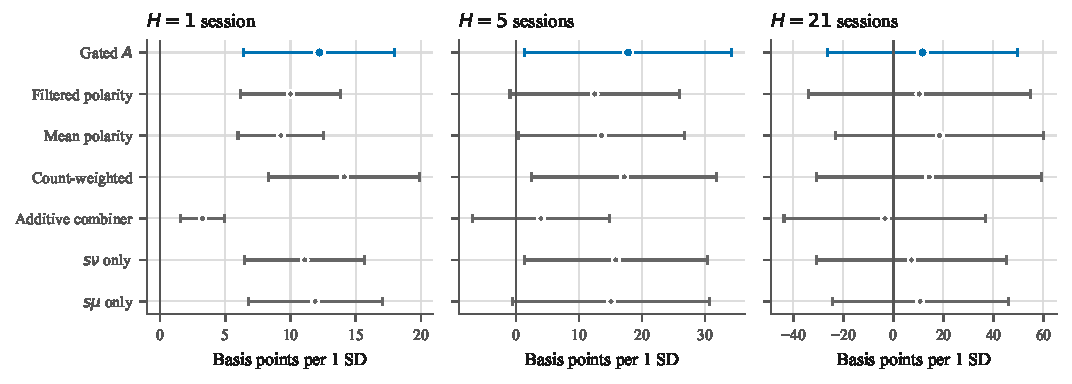
\includegraphics[width=\textwidth]{figures/fig2_univariate.pdf}
\caption{Forward-return coefficient on each aggregator, in basis points per one
standard deviation of signal, with 95\% intervals from two-way clustered standard
errors. The gated signal is highlighted; the alternatives are shown in neutral
ink.}
\label{fig:univariate}
\end{figure}

\subsection{The nested horse race}\label{sec:horserace}

Entering all four terms together (Table~\ref{tab:horserace}) was intended to be
the sharp test: multiplicative gating predicts that the product loads and absorbs
the lower-order terms. What happens instead is that nothing is individually
identified. At one session the gated aggregate carries the largest coefficient
($16.3$ basis points) but only $t=1.58$, while mean polarity falls to $t=1.26$ and
the two single-axis ablations take opposite signs. At five and twenty-one sessions
the coefficients grow large and alternate in sign --- $+50.3$ for the product
against $-36.2$ for the materiality gate at five sessions --- with $|t|<2$
throughout.

This pattern is diagnostic of collinearity, not of a hidden effect, and
Section~\ref{sec:descriptive} already told us why: with $\nu$ and $\mu$ correlated
at $0.871$ and all four regressors built from the same polarity, the design matrix
is close to singular and the individual coefficients are not separately estimable.
We therefore decline to read anything into the sign or size of any single term
here. The honest conclusion from this table is a statement about what the data
\emph{cannot} answer: on this corpus, the nested horse race does not have the
power to distinguish the product from its components.

\begin{table}[htbp]
\caption{The nested horse race. All four terms enter one regression, so each
coefficient is the marginal contribution of that term given the others.
Multiplicative gating predicts that the gated signal loads and absorbs the
lower-order terms. Regressors standardised; two-way clustered $t$-statistics.}
\label{tab:horserace}
\begin{tabular}{@{}lcccccc@{}}
\toprule
 & \multicolumn{2}{c}{$H=1$} & \multicolumn{2}{c}{$H=5$} & \multicolumn{2}{c}{$H=21$} \\
Term & bps & $t$ & bps & $t$ & bps & $t$ \\
\midrule
Mean polarity & 6.2 & 1.26 & 23.1$^{*}$ & 1.92 & 85.5$^{*}$ & 1.76 \\
Novelty gate only ($s\nu$) & -9.1 & -1.30 & -15.2 & -0.63 & -103.8$^{*}$ & -1.77 \\
Materiality gate only ($s\mu$) & 0.4 & 0.05 & -36.2 & -1.25 & -64.7 & -0.59 \\
Gated signal $A$ & 16.3 & 1.58 & 50.3 & 1.33 & 111.8 & 0.98 \\
\botrule
\end{tabular}
\end{table}


\subsection{Free exponents}\label{sec:exponents}

The horse race cannot separate the terms, but the exponent grid can ask a cleaner
question, because it varies the functional form directly instead of trying to
identify collinear regressors. Remark~\ref{rem:notpinned} left
$\alpha$ and $\beta$ free; here we estimate them by sweeping
$s\,\nu^{\alpha}\mu^{\beta}$ over $[0,2]^2$ and reading off the information
coefficient of the resulting aggregate.

The answer is unambiguous and it is not the one the unit-exponent product
predicts. At one session the grid maximum sits at
$\alpha=\BestAlphaHOne$, $\beta=\BestBetaHOne$ with IC $\BestICHOne$: the
materiality exponent is estimated at \emph{exactly zero}. The unit-exponent
product assumed by Eq.~\eqref{eq:signal} scores $\UnitICHOne$, and switching the
gates off altogether --- $\alpha=\beta=0$, which collapses the aggregate to plain
mean polarity --- scores $\PureICHOne$. At five sessions the maximum is the
no-gating corner itself, $\alpha=\beta=0$ with IC $\BestICHFive$, against
$\UnitICHFive$ for the unit-exponent product: there, gating is not merely
unhelpful but actively harmful.

Two conclusions follow. First, $H_0\!:\alpha=\beta=1$ is rejected, and rejected in
the direction of the null model rather than toward some richer weighting. Second,
and more important, the entire surface spans only $0.0201$ to $0.0225$ in
information coefficient (Figure~\ref{fig:exponents}). The objective is nearly flat
in the exponents, so the choice of gating weights --- including the choice not to
gate --- moves predictive accuracy by an amount that is small relative to its own
sampling error. That flatness, rather than the location of any maximum, is the
finding, and it is why every comparison in Section~\ref{sec:selective} lands
inside its confidence interval.

\begin{figure}[htbp]
\centering
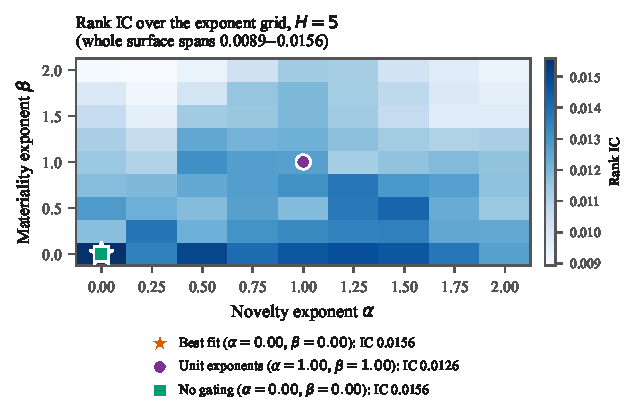
\includegraphics[width=0.62\textwidth]{figures/fig4_exponents.pdf}
\caption{Information coefficient of the aggregate built from
$s\,\nu^{\alpha}\mu^{\beta}$ over a grid of exponents. The unit-exponent product
assumed by Eq.~\eqref{eq:signal} is marked, as is the empirical maximum;
Remark~\ref{rem:notpinned} explains why the axioms leave this an open question.}
\label{fig:exponents}
\end{figure}

\subsection{Selective forecasting with and without the gated signal}\label{sec:selective}

This is the experiment the framework has to pass, and the one earlier versions of
this study did not run: the conviction gate is fitted twice on identical
walk-forward folds, once on price features alone and once on price features plus
the gated text signal, and the reported quantity is the difference between them.

There is no difference. Adding $A$ moves precision at a fixed $10\%$ coverage by
$\GapPriceHOne$ percentage points at one session
(95\% CI \GapPriceCIHOne, $p=\GapPricePHOne$), $\GapPriceHFive$ points at five
sessions (\GapPriceCIHFive, $p=\GapPricePHFive$) and $\GapPriceHTwentyOne$ points
at twenty-one (\GapPriceCIHTwentyOne, $p=\GapPricePHTwentyOne$). Against
relevance-filtered polarity rather than against price alone the gaps are
$\GapRelfHOne$, $\GapRelfHFive$ and $\GapRelfHTwentyOne$ points. Every interval
contains zero, and the point estimates change sign across horizons. The
risk--coverage curves of Figure~\ref{fig:riskcov} say the same thing without
reference to any threshold: the curves for the four feature sets are
indistinguishable over the whole coverage range, and their AURCs differ in the
third decimal.

One result in Table~\ref{tab:gate} does not fit the pattern, and we report it
because it is the most interesting thing in the table. The \emph{text-only} model
--- no price features at all --- achieves the best AURC at both short horizons
($\AurcAHOne$ against $\AurcPriceHOne$ for price-only at one session, and $0.468$
against $\AurcPriceHFive$ at five) and the best precision at five sessions
($55.3\%$ against $\PrecPriceHFive\%$ for price-only, on a $\BaseRateHFive\%$ base
rate). The headlines therefore carry decision-relevant information that the price
features do not, and a learner given the text alone finds it. What the learner
cannot do is exploit that information \emph{once price features are also
available}: the combined model is no better than price alone. Whether this
reflects a genuine redundancy or a failure of the gradient-boosted learner to
allocate capacity to a weak, sparse feature beside strong dense ones, we cannot
determine from these data, and we would not want a reader to take the first
explanation for granted.

\begin{table}[htbp]
\caption{Selective forecasting with and without the gated text signal. Precision
is the realised up-rate of the most confident 10\% of out-of-sample predictions,
a fixed coverage that makes the variants comparable without reference to any
tuned threshold; AURC is the area under the risk--coverage curve, for which lower
is better. All figures are pooled over walk-forward test years. The lower panel
bootstraps the precision gap by resampling whole dates.}
\label{tab:gate}
\small
\begin{tabular}{@{}lcccccc@{}}
\toprule
 & \multicolumn{2}{c}{$H=1$} & \multicolumn{2}{c}{$H=5$} & \multicolumn{2}{c}{$H=21$} \\
Feature set & Prec. & AURC & Prec. & AURC & Prec. & AURC \\
\midrule
Price $+$ gated signal $A$ & 51.5 & 0.479 & 52.4 & 0.472 & 59.7 & 0.458 \\
Price $+$ filtered polarity & 51.4 & 0.482 & 53.8 & 0.472 & 59.1 & 0.460 \\
Price $+$ mean polarity & 51.2 & 0.484 & 53.4 & 0.470 & 59.3 & 0.459 \\
Price only & 51.2 & 0.485 & 54.0 & 0.473 & 59.0 & 0.457 \\
Text only & 52.8 & 0.479 & 55.3 & 0.468 & 58.9 & 0.462 \\
\midrule
Always-up base rate & \multicolumn{2}{c}{51.8\%} & \multicolumn{2}{c}{53.3\%} & \multicolumn{2}{c}{54.9\%} \\
\botrule
\end{tabular}

\vspace{0.6em}
\begin{tabular}{@{}lccc@{}}
\toprule
Precision gap at 10\% coverage & Estimate (pp) & 95\% CI & $p$ \\
\midrule
$H=1$, vs.\ price only & +0.37 & [-1.26, +1.96] & 0.685 \\
$H=1$, vs.\ filtered polarity & +0.07 & [-1.70, +1.83] & 0.938 \\
$H=1$, vs.\ mean polarity & -0.05 & [-2.23, +2.14] & 0.948 \\
$H=5$, vs.\ price only & -1.23 & [-3.52, +1.13] & 0.322 \\
$H=5$, vs.\ filtered polarity & -0.83 & [-3.10, +1.40] & 0.482 \\
$H=5$, vs.\ mean polarity & -0.65 & [-2.96, +1.64] & 0.587 \\
$H=21$, vs.\ price only & +0.01 & [-0.74, +0.72] & 1.000 \\
$H=21$, vs.\ filtered polarity & +0.37 & [-0.23, +0.97] & 0.252 \\
$H=21$, vs.\ mean polarity & +0.28 & [-0.32, +0.84] & 0.345 \\
\botrule
\end{tabular}
\end{table}


\begin{figure}[htbp]
\centering
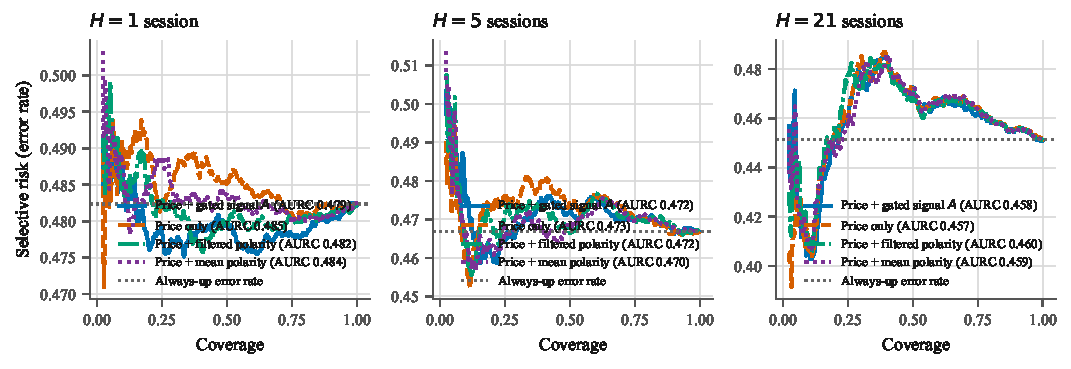
\includegraphics[width=\textwidth]{figures/fig3_risk_coverage.pdf}
\caption{Risk--coverage curves for the walk-forward selective forecaster. Each
curve traces the error rate accepted at every coverage level, so the comparison
does not depend on the choice of any single conviction threshold; the area under
each curve (AURC, lower is better) appears in the legend.}
\label{fig:riskcov}
\end{figure}

\subsection{Deployment evidence: coverage and calibration}\label{sec:live}

The results above concern the text stage. The decision stage was studied on the
deployed Indian system, where the evidence is of a different kind: not whether a
signal predicts, but whether a system in production tells the truth about its own
uncertainty.

It did not. Between 19 April and 12 June 2026 the system issued and later resolved
621 price-interval forecasts on seven NSE large caps, each carrying a nominal
$90\%$ interval with a median half-width of $5.6\%$ of price. Had those intervals
been calibrated, about $90\%$ would have contained the realised price; empirical
coverage was $70.7\%$, a $19.3$ percentage-point shortfall
(Table~\ref{tab:live}, Figure~\ref{fig:deployment}(a)). Most forecasts sat at the
ten-day horizon, where coverage was $69.2\%$ over 575 resolved forecasts. Nothing
in the pipeline noticed, which is the point: overconfidence is silent unless
somebody scores it.

The directional head failed in the same direction and for a diagnosable reason.
It reported next-day up-probabilities clustered near $0.80$ against a realised
accuracy near $0.51$, giving an expected calibration error of $0.345$ and a Brier
score above $0.366$ --- worse than predicting $0.5$ every time. The cause was the
stacking domain mismatch of Section~\ref{sec:calib}, and the three-stage repair
cut expected calibration error from $0.345$ to $0.049$ while leaving accuracy
untouched. Calibration changed what the model \emph{said about its confidence},
not what it predicted, which is precisely the distinction the framework insists
on.

With probabilities pulled back to the base rate, the walk-forward conviction gate
on the 54-name deployment universe (2018--2026, 91{,}471 training rows and 50{,}272
out-of-sample rows) settles at $\tau^\star=0.63$ and fires on $5.6\%$ of
observations, abstaining on the rest. The fired bucket realises $60.6\%$
directional precision against a $58.0\%$ always-up base rate over $2{,}840$ pooled
calls: a $2.6$ point edge with a $95\%$ binomial interval of $58.8$ to $62.4\%$.
We do not over-read it. Per-year counts are small, the swing from $+10.8$ points
in 2025 to $-2.4$ in 2024 is within sampling noise
(Figure~\ref{fig:deployment}(b)), and the ranking area under the curve is about
$0.47$, so what edge exists lives in the high-conviction tail and not in the
ordering. Crucially for this paper, \emph{this gate contains no text feature at
all}: it is evidence that calibrated abstention is worth building, not evidence
for the decomposition.

\begin{table}[htbp]
\caption{Deployment evidence from the live forecast ledger. Every interval
carries a nominal 90\% level. Panel B reports the walk-forward conviction gate on
the 54-name deployment universe, where precision is the realised up-rate of the
fired high-conviction bucket and the base is the unconditional always-up rate.}
\label{tab:live}
\begin{tabular}{@{}lccc@{}}
\toprule
\multicolumn{4}{@{}l}{\textit{Panel A: interval coverage by horizon}} \\
Horizon & Resolved forecasts & Nominal & Empirical \\
\midrule
5 trading days  & 8   & 90.0\% & 100.0\% \\
10 trading days & 575 & 90.0\% & 69.2\%  \\
20 trading days & 38  & 90.0\% & 86.8\%  \\
\textbf{All}    & \textbf{621} & \textbf{90.0\%} & \textbf{70.7\%} \\
\botrule
\end{tabular}

\vspace{0.6em}
\begin{tabular}{@{}lcccc@{}}
\toprule
\multicolumn{5}{@{}l}{\textit{Panel B: walk-forward conviction gate by test year}} \\
Test year & Fires & Fired precision & Always-up base & Edge (pp) \\
\midrule
2022 & 365 & 61.6\% & 54.0\% & $+7.6$ \\
2023 & 290 & 68.3\% & 65.3\% & $+3.0$ \\
2024 & 932 & 53.3\% & 55.7\% & $-2.4$ \\
2025 & 822 & 69.0\% & 58.2\% & $+10.8$ \\
2026 & 431 & 54.5\% & 47.1\% & $+7.4$ \\
\textbf{Pooled} & \textbf{2{,}840} & \textbf{60.6\%} & \textbf{58.0\%} & \textbf{$+2.6$} \\
\botrule
\end{tabular}
\footnotetext{The pooled base is the unconditional always-up rate over all
out-of-sample rows, not the fires-weighted mean of the yearly bases (55.9\%); the
pooled edge is therefore the more conservative of the two comparisons.}
\end{table}


\begin{figure}[htbp]
\centering
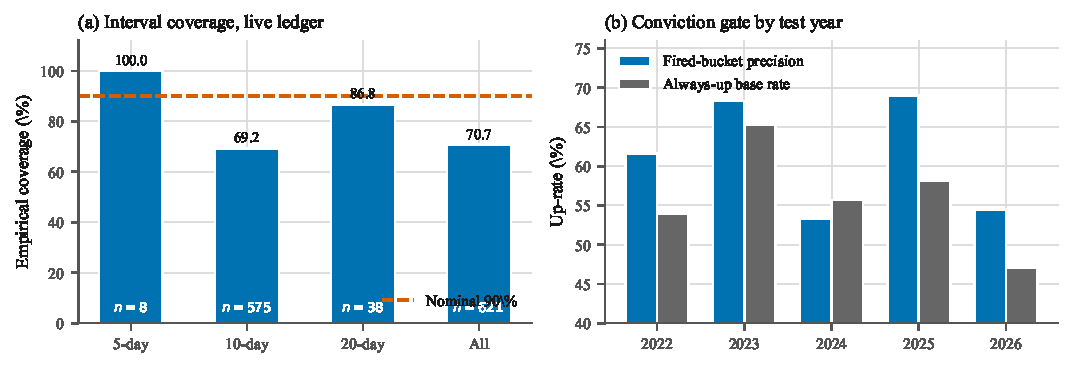
\includegraphics[width=\textwidth]{figures/fig5_deployment.pdf}
\caption{Deployment evidence. (a) Empirical coverage of nominal 90\% price
intervals on the live ledger, by horizon. (b) Fired-bucket precision of the
conviction gate against the always-up base rate, by walk-forward test year, at
roughly a 5.6\% firing rate.}
\label{fig:deployment}
\end{figure}

\subsection{Robustness}\label{sec:robust}

A null result is only worth reporting if it is not an artefact of the analyst's
choices, so we varied the three that matter.

\emph{The materiality floor.} Sweeping $\mu_0$ from $0$ (no floor) to $0.40$
leaves the one-session coefficient on $A$ between $12.0$ and $12.2$ basis points
with $t$ between $3.97$ and $4.14$. The floor simply does not bind on the
conclusion, which is what one expects when the exponent on materiality is
estimated at zero. One detail cuts the other way and we note it: at five sessions
the information coefficient rises from $0.013$ at $\mu_0=0$ to $0.025$ at
$\mu_0=0.25$ and above, with the Newey--West $t$ going from $1.24$ to $2.25$. A
\emph{hard relevance filter} thus helps where multiplicative weighting does not
--- consistent with the exponent surface, and consistent with what practitioners
already do with vendor relevance scores.

\emph{Overlapping versus non-overlapping windows.} Using every session rather than
every $H$-th weakens the five-session result from $17.8$ basis points ($t=2.12$)
to $8.9$ ($t=1.68$), in the direction that the overlapping-observation literature
predicts. We report non-overlapping windows as the primary specification for that
reason; neither choice changes the comparison between aggregators, which is what
the paper turns on.

\emph{Quiet sessions.} Restricting the panel to symbol-sessions that carry scored
news is the primary specification, since including quiet sessions pads the sample
with rows where every text aggregator is identically zero and can only dilute any
difference between them.

\emph{Repeatability of the instrument.} Cross-model agreement is reported in
Section~\ref{sec:reliability}. We regard it as the weakest link in the measurement
chain and the first thing a replication should attack.

% =============================================================================
\section{Discussion}\label{sec:discussion}
% =============================================================================

\subsection{Why the decomposition did not pay}

Section~\ref{sec:validity} lets us be specific rather than speculative, and the
answer has two parts.

\emph{One axis is not measuring what it is named.} Novelty fails its external
criterion: it does not track mechanical staleness beyond what materiality already
tracks, its profile against mechanical novelty is the same curve as materiality's,
and it is non-monotonic besides. Materiality, by contrast, passes decisively,
predicting absolute market-adjusted returns at $\AbsRetMuT$ standard errors. So
the $0.871$ correlation is not the world telling us that novel news is material
news; it is one latent ``importance'' judgement being reported twice under two
labels, only one of which corresponds to something external. A product of two
gates cannot behave like a two-gate product when only one gate exists.

\emph{The surviving axis carries the wrong quantity for the task.} Materiality is
by definition about magnitude irrespective of sign, and that is exactly how it
behaves. Multiplying it into a \emph{signed} signal, as Eq.~\eqref{eq:signal}
does, asks a magnitude variable to sharpen a direction forecast, which it has no
means of doing. This is the cleanest reading of the zero materiality exponent in
Section~\ref{sec:exponents}, and it points somewhere constructive: the same
decomposition aimed at a volatility or absolute-return target, where materiality's
information is the relevant kind, is a genuinely different experiment and one we
have not run.

\emph{Attenuation remains a live secondary concern.} Cross-model intraclass
correlations are $\ICCS$ for polarity but only $\ICCNu$ for novelty, and the
product inherits $0.601$; multiplying noisy factors compounds their noise, so
classical errors-in-variables would bias the measured contribution of gating
toward zero. We cannot rule this out, and it is a further reason the framework
deserves a rematch with a better instrument rather than a dismissal. What it does
not license is treating the null as a measurement artefact by assumption --- and
in any case attenuation cannot explain why novelty points the \emph{wrong way} on
absolute returns, which is a validity failure and not a noise problem.

Beyond that, note what did survive.
The additive combiner performed worst of all the aggregators, so collapsing the
axes by addition is clearly wrong; and a \emph{hard} materiality filter improved
the five-session information coefficient from $0.013$ to $0.025$ where
multiplicative weighting did not. Read together, these say that relevance
information is worth using as a \emph{filter} --- decide which items to look at ---
but not as a continuous multiplicative \emph{weight} on the ones that survive. The
practitioner convention of thresholding a vendor relevance score, which we set out
to improve on, appears to be the right call.

\subsection{What this means for practice and for the literature}

For a practitioner the recommendation is unglamorous and specific: filter on
relevance, then average polarity. The elaboration we proposed costs an extra
language-model call per headline, introduces a second noisy axis, and returns
nothing measurable. Where a language model does earn its keep is upstream, in
deciding which items to consider at all.

For the literature, the more useful contribution may be the measurement rather
than the null. That a competent language model, given careful definitions and four
numerical anchors per axis, returns novelty and materiality scores correlated at
$0.871$ --- of which only the materiality channel survives an external validity
check --- is a fact about these instruments that anyone building multi-axis text
features should know before designing around an assumed separation. Prompt-based
scores are not independent merely because the prompt asks for independent things,
and asking a model for $k$ conceptually distinct scores does not guarantee $k$
distinct measurements. The cheap diagnostic we would urge on anyone in this
position is the one in Section~\ref{sec:validity}: name an external criterion for
each axis \emph{before} building features from it, and check that each axis tracks
its own criterion and not merely its neighbour's.

We also note one asymmetry worth following up. The text-only model beat the
price-only model on AURC at both short horizons, while the combined model beat
neither. Weak, sparse, noisy features sitting beside strong dense ones are exactly
the case where a gradient-boosted learner is known to underuse them, so the right
conclusion is not that the text is redundant but that we have not shown how to
combine it. That is a question about model architecture rather than about the
decomposition, and it is where we would look next.

\subsection{What the design buys, and what it costs}

Every result in this paper turns on one trade-off. The text-stage veto refuses
stale or immaterial items and the decision-stage gate stays out on most names, so
the system gives up commenting on everything in exchange for the right to be
believed on the little it flags. That trade is not free, and the risk--coverage
curves of Figure~\ref{fig:riskcov} are the honest way to price it: they show what
error rate is bought at every level of coverage rather than at the single
operating point that happens to flatter the method.

Nothing in Section~\ref{sec:model} is specific to equities. Any stream of
timestamped textual events feeding a decision has the same three axes, and the
same failure mode when they are collapsed into one score: triage of clinical
alerts, operations tickets and content-moderation queues all conflate ``how bad''
with ``how new'' and ``how consequential''. The decision-stage half of the design
is an instance of selective classification \citep{chow1970,geifman2017}, here
paired with a probability whose calibration was repaired rather than assumed, and
the interval-coverage failure of Section~\ref{sec:live} is exactly the problem
distribution-free methods \citep{angelopoulos2023} are built for.

\subsection{Limitations}\label{sec:limits}

Five limitations bound what may be concluded, and we would rather state them than
have them found.

\emph{The validation market is not the deployment market.} The decomposition is
tested on US headlines and the deployed system trades Indian equities. We report
no result that crosses that boundary, but the reader should not read the US panel
as evidence about NSE microstructure, disclosure regimes or news supply, all of
which differ.

\emph{The axes are judgements, and one of them did not survive validation.}
Anchoring the prompt tightens the scores and Section~\ref{sec:reliability}
quantifies their repeatability, but repeatability is not validity: a scorer can be
perfectly consistent and consistently wrong, which is close to what
Section~\ref{sec:validity} finds for novelty. Every result about gating is
therefore a joint test of the decomposition and of this particular instrument, and
a differently worded rubric, a larger model, or a two-stage prompt that scores the
axes independently might separate them where ours did not. We consider that the
single most valuable follow-up.

\emph{The external criteria are proxies.} Lexical similarity over a thirty-day
window is a serviceable but crude stand-in for what the market already knew, and
absolute return is a noisy realisation of an event's true importance. A criterion
failure is therefore weaker evidence than a criterion success: materiality passing
is strong evidence it measures something, whereas novelty failing is consistent
with both a bad axis and a bad proxy.

\emph{The comparison is against feasible baselines, not against a vendor feed.}
The most informative comparison would be against a commercial relevance and
novelty product on the same headlines. We do not have a licence for one, so the
relevance-filtered polarity baseline is our best available stand-in for what a
practitioner would actually deploy.

\emph{The live ledger is young and small.} Two months and seven names is a
snapshot of coverage behaviour, not a stationary law, and the live directional
sample is far too small to support a claim about skill. That is why the live
evidence in this paper is confined to calibration and interval coverage, where
621 resolved forecasts is enough to say something, and the claims about selection
rest on walk-forward evidence instead.

\emph{Selection and multiple testing.} We report several horizons, several
aggregators and several feature sets. The risk--coverage curves and the
non-overlapping-window specification remove the most common sources of
optimism, and differences between models carry bootstrap intervals, but a reader
who wants a single number with a family-wise guarantee should apply a stepdown
correction \citep{romano2005} to the horse-race column and read the result
accordingly. Financial machine learning has a well-documented tendency to
discover edges that do not survive \citep{bailey2017,harvey2016}, and we would
rather our estimates be read with that prior in mind.

% =============================================================================
\section{Conclusion}\label{sec:conclusion}
% =============================================================================

A textual event carries direction, surprise and consequence, and there is a clean
argument that these should combine multiplicatively: the product makes freshness
and relevance preconditions for influence, it caps the signal at its weakest
factor, and under continuity, monotonicity and ratio-scale separability it is the
form the axes must take, up to exponents the axioms leave free.

Measured against real data, the argument does not pay. On \ScoredHeadlines\
headlines covering \NCompanies\ companies, the gated aggregate predicts
market-adjusted returns at short horizons but no better than mean polarity,
count-weighted polarity or relevance-filtered polarity; estimating the exponents
freely puts materiality's at zero and, at five sessions, collapses the aggregate
to plain polarity; and adding the gated signal to a walk-forward selective
forecaster moves precision at fixed coverage by between $-1.2$ and $+0.4$
percentage points, with every interval containing zero.

The explanation is in the measurement rather than in the market, and it is
specific. Novelty and materiality, as an instruction-tuned model scores them,
correlate at $0.871$; validated against external criteria, only materiality
survives, predicting absolute market-adjusted returns at $\AbsRetMuT$ standard
errors, while novelty fails to track mechanical staleness beyond what materiality
already tracks and enters absolute returns with the wrong sign. The three-axis
decomposition is empirically a two-axis one, and the axis that does measure
something measures \emph{magnitude}, which a signed product has no way to exploit.

Two things do survive. Adding the axes is worse than multiplying them, so the
case against additive combination stands. And using relevance as a hard filter
rather than a continuous weight improves the five-session information coefficient
from $0.013$ to $0.025$ --- which is what practitioners already do with vendor
relevance scores, now with evidence behind it. Separately, on the deployment side,
nominal $90\%$ intervals covered $70.7\%$ of live outcomes, a three-stage
recalibration cut expected calibration error from $0.345$ to $0.049$ without
touching accuracy, and a conviction gate abstaining on $94\%$ of names raised the
thirty-day hit rate to $60.6\%$ against a $58.0\%$ base --- evidence that
calibrated abstention is worth building, independent of anything the text stage
does.

The framework is intuitive and will be proposed again. We think the more useful
contribution is the record of what happened when it was built, instrumented and
tested: the decomposition is measurable, the veto provably and visibly works, and
it buys nothing over averaging polarity --- for reasons that are now diagnosed
rather than guessed at. Two experiments follow directly and neither is run here.
An instrument whose novelty channel passes an external validity check would give
the framework the fair test it has not yet had; and pointing the same
decomposition at a volatility or absolute-return target, where materiality's
information is of the relevant kind, asks the question the signed formulation
cannot. The measurements reported here are designed to make both possible, and to
make it costly for the next version of this idea to be adopted without them.

% =============================================================================
\backmatter

\bmhead{Acknowledgements}
The authors thank Fr.\ C.\ Rodrigues Institute of Technology for computing
support.

\section*{Declarations}

\paragraph{Funding} No external funding was received for this work.

\paragraph{Competing interests} The authors declare no competing interests.

\paragraph{Availability of data and materials} The FNSPID news corpus is publicly
available \citep{dong2024}; price data are public end-of-day records. The scored
axis values, the derived panel, the analysis code and the live forecast ledger
underlying the reported tables and figures are available from the corresponding
author on reasonable request.

\paragraph{Use of generative artificial intelligence} An instruction-tuned
language model is used as a measurement instrument \emph{within the system under
study}, scoring headlines along the three axes from the anchored prompt of
Section~\ref{sec:scoring}; those outputs are persisted for audit. During
manuscript preparation a large language model was used solely to improve language
and readability. No generative tool produced the data, results, figures or
interpretations, and the authors take full responsibility for the content.

\paragraph{Authors' contributions} Both authors contributed to the study
conception and design, analysis and interpretation. Both authors read and
approved the final manuscript.

\paragraph{Author ORCIDs}
Anandkumar Pardeshi \textemdash\ \url{https://orcid.org/0000-0003-2806-3305};
Sujata Deshmukh \textemdash\ \url{https://orcid.org/0000-0001-9893-6947}.

\bibliography{refs}

\end{document}
